\noindent

\includegraphics[height=1.25cm]{images/pictograms/benchmark}

\includegraphics[height=1.25cm]{images/pictograms/FDM}

%%%%%%%%%%%%%%%%%%%%%%%%%%%%%%%%%%%%%%%%%%%%%%%%%%%%%%%%%%%%%%%%%%%%%%%%%%%%%%%%%%%%%%%%%%%%%%%%%%%

\begin{flushright} {\tiny {\color{gray} python\_codes/fieldstone\_157/text.tex}} \end{flushright}

%\lstinputlisting[language=bash,basicstyle=\small]{python_codes/template_keywords.key}

\par\noindent\rule{\textwidth}{0.4pt}

\begin{center}
\inpython
{\small Code: \url{https://github.com/cedrict/fieldstone/tree/master/python_codes/fieldstone_157}}
\end{center}

\par\noindent\rule{\textwidth}{0.4pt}

%{\sl This stone was developed in collaboration with Donald Duck}. \index{contributors}{D. Duck}

%\par\noindent\rule{\textwidth}{0.4pt}

%%%%%%%%%%%%%%%%%%%%%%%%%%%%%%%%%%%%%%%%%%%%%%%%%%%%%%%%%%%%%%%%%%%%%%%%%%%%%%%%%%%%%%%%%%%%%%%%%%%

We start from the 1D diffusion equation
\[
\frac{\partial T}{\partial t} = \kappa \frac{\partial^2 T}{\partial x^2}
\]
We then discretise the space derivative by means of a centered stencil:
\[
\frac{\partial T_i}{\partial t} = \kappa \frac{T_{i+1}-2T_i+T_{i-1}}{h^2}
\]
where $i=0,nnx-1$.

Traditionallly we would continue by discretising the time derivative and 
end up with an explicit, implit or hybrid scheme (e.g. Crank-Nicolson). 
However in this case we stop here and in essence we have replaced a PDE by 
a set of ODEs, one per node in the domain,
which can be written as follows:
\[
\frac{\partial \vec{T}}{\partial t} = \vec{\cal F}(\vec{T}) 
\] 
where $\vec{T}$ contains all the temperature values at the nodes.

In \textcite{boudreau} (from which this idea is borrowed, see p328 )
this method is called the Method of Lines (MoL)\footnote{\url{http://var.scholarpedia.org/article/Method_of_lines}} and we read:
``
There are significant advantages in solving diagenetic equations\footnote{These
are advection-diffusion-reaction equations.} by the MoL: 
i) stiff problems caused by fast reactions are handled readily; 
ii) highly nonlinear problems can be solved with no fuss; 
iii) the initial guess is not all that important when solving for the steady state; 
iv) this procedure is usually very stable and convergent; 
v) the number of space dimensions is irrelevant; and 
vi) both transient and steady-state problems can be solved.
''
The method lends itself to using any kind of ODE integrator (RK methods and more, 
see Section~\ref{MMM-ss:rkm}).

The domain is a segment of length $L_x=1$. There are $nnx=101$ equidistant nodes. 
The initial temperature is set to $T(x,t=0)=0.123$ everywhere 
except at the ends where it is set to $T_{left}=1$ and $T_{right}=0$.
The heat diffusivity is set to $\kappa=0.01$. The model is run until $t_{final}=100$.
The time step is computed as $\delta t=h^2/2\kappa$ where $h=L_x/(nnx-1)$.
To start with the time derivative will be dealt with by means of a 1st order
Euler step:
\[
\frac{\partial T}{\partial t} \simeq \frac{T^{n+1}-T^n}{\delta t}
\]
This then results in a FTCS algorithm.
In a second step, we may wish to use the {\python solve\_ivp} 
function\footnote{\url{https://docs.scipy.org/doc/scipy/reference/generated/scipy.integrate.solve_ivp.html}}
which gives access to 5 methods: RK23, RK45 (default) DOP853, BDF and Radau.

\begin{lstlisting}
soln = solve_ivp(F,(0,tfinal),T0,args=(kappa,),method=RKmethod ,max_step=maxdt)
\end{lstlisting}

In our case the ODEs at hand are linear and not stiff, so that 
there is in fact no need for such high-order methods.
I have verified that this works but since it yields virtually identical 
results to the 1st order scheme I am not showing any results obtained with this function in what follows.

%..............................
\subsubsection*{option \#1}

If Dirichlet boundary conditions are prescribed at both ends of the domain, 
then the temperature is constant there in time and then $\frac{\partial T_i}{\partial t}=0$ there.
This translates as follows:
\begin{lstlisting}
   def F(t,T,kappa):
       dT_dt=np.zeros(nnx,dtype=np.float64)
       for i in range(0,nnx):
           if i==0:
              dT_dt[i]=0
           elif i==nnx-1: 
              dT_dt[i]=0
           else:
              dT_dt[i]=kappa*(T[i+1]-2*T[i]+T[i-1])/h**2
       return dT_dt
\end{lstlisting}

The time evolution of the temperature is shown hereunder and we find that 
it converges to the expected analytical solution $t(x)=1-x$.

\begin{center}
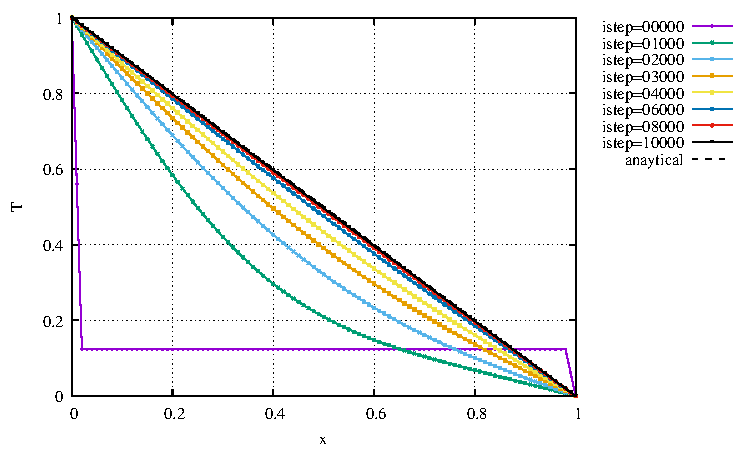
\includegraphics[width=12cm]{python_codes/fieldstone_157/results/option1/T.pdf}
\end{center}

%..............................
\subsubsection*{option \#2}

If we now assume a Dirichlet boundary condition at $x=0$ and a Neumann boundary condition 
on the right (i.e. $\partial T/\partial x=0$, or no heat flux), we must look closer at what is going on 
on this node. 
We start by writing the second-order derivative as follows (fully backward, since
a standard centered stencil would involve a node to the right of the node 
under consideration but there is none):
\[
\frac{\partial T_i}{\partial t} = \kappa \frac{T_{i}-2T_{i-1}+T_{i-2}}{h^2}
\]
On this node the boundary condition writes (again, a backward formulation is necessary)
\[
\frac{T_i-T_{i-1}}{h}=0
\]
which, when incorporated in the equation above, leads to:
\[
\frac{\partial T_i}{\partial t} 
= \kappa \frac{(T_{i}-T_{i-1})-T_{i-1}+T_{i-2}}{h^2}
= \kappa \frac{-T_{i-1}+T_{i-2}}{h^2}
\]
The function $\vec{\cal F}$ then writes
\begin{lstlisting}
   def F(t,T,kappa):
       dT_dt=np.zeros(nnx,dtype=np.float64)
       for i in range(0,nnx):
           if i==0:
              dT_dt[i]=0
           elif i==nnx-1: 
              dT_dt[i]=kappa*(-T[i-1]+T[i-2])/h**2
           else:
              dT_dt[i]=kappa*(T[i+1]-2*T[i]+T[i-1])/h**2
       return dT_dt
\end{lstlisting}

The steady-state solution is actually $T(x)=1$ and we find that our solution slowly converges towards it
while maintaining a zero derivative on the right side of the domain.
\begin{center}
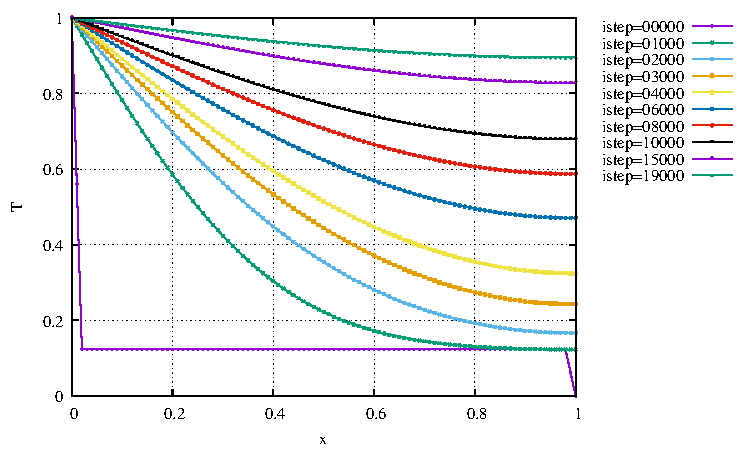
\includegraphics[width=12cm]{python_codes/fieldstone_157/results/option2/T.pdf}
\end{center}






 
